\documentclass[10pt]{article}
\usepackage{graphicx}
\usepackage{geometry}
\usepackage{indentfirst}
\usepackage{amsmath}
\usepackage{amssymb}
\usepackage{booktabs}
\usepackage{setspace}
\usepackage{listings}
\usepackage{subfig}
\usepackage{hyperref}
\usepackage{color}
\usepackage[table]{xcolor}
\usepackage[nottoc,notlot,notlof]{tocbibind}

\definecolor{mygreen}{rgb}{0,0.6,0}
\definecolor{mygray}{rgb}{0.5,0.5,0.5}
\definecolor{mymauve}{rgb}{0.58,0,0.82}

\geometry{
    letterpaper,
    left = 0.75in,
    right = 0.75in,
    top = 30mm,
    bottom = 30mm
}

\lstset{ %
  backgroundcolor=\color{white},   % choose the background color; you must add \usepackage{color} or \usepackage{xcolor}
  basicstyle=\footnotesize,        % the size of the fonts that are used for the code
  breakatwhitespace=false,         % sets if automatic breaks should only happen at whitespace
  breaklines=true,                 % sets automatic line breaking
  captionpos=b,                    % sets the caption-position to bottom
  commentstyle=\color{mygreen},    % comment style
  deletekeywords={...},            % if you want to delete keywords from the given language
  escapeinside={\%*}{*)},          % if you want to add LaTeX within your code
  extendedchars=true,              % lets you use non-ASCII characters; for 8-bits encodings only, does not work with UTF-8
  frame=single,                    % adds a frame around the code
  keepspaces=true,                 % keeps spaces in text, useful for keeping indentation of code (possibly needs columns=flexible)
  keywordstyle=\color{blue},       % keyword style
  language=C++,                 % the language of the code
  morekeywords={*,...},            % if you want to add more keywords to the set
  numbers=left,                    % where to put the line-numbers; possible values are (none, left, right)
  numbersep=5pt,                   % how far the line-numbers are from the code
  numberstyle=\tiny\color{mygray}, % the style that is used for the line-numbers
  rulecolor=\color{black},         % if not set, the frame-color may be changed on line-breaks within not-black text (e.g. comments (green here))
  showspaces=false,                % show spaces everywhere adding particular underscores; it overrides 'showstringspaces'
  showstringspaces=false,          % underline spaces within strings only
  showtabs=false,                  % show tabs within strings adding particular underscores
  stepnumber=2,                    % the step between two line-numbers. If it's 1, each line will be numbered
  stringstyle=\color{mymauve},     % string literal style
  tabsize=2,                       % sets default tabsize to 2 spaces
  title=\lstname                   % show the filename of files included with \lstinputlisting; also try caption instead of title
}

\newcommand{\beac}{\textbf{Beacon }}
\newcommand{\doc}[1]{Dr.\@ #1}

\captionsetup{belowskip=12pt,aboveskip=12pt}

% \textit{blastp}
% Intel \textsuperscript{\textregistered} Xeon\textsuperscript{\textregistered} 
%  Intel \textsuperscript{\textregistered} Xeon Phi\texttrademark \hspace*{2pt}
% Intel \textsuperscript{\textregistered} VTune\texttrademark \hspace*{2pt}

% \begin{figure}[!htbp]
% \centering
% \:graphics[scale=0.4]{./Images/mpi_model_4.eps}
% \caption{HPC-BLAST MPI layer.}
%\end{figure}

% \begin{figure}[!htbp]
% \centering
% \includegraphics[scale=0.4]{./Images/thread_model.eps}
% \caption{HPC-BLAST thread layer.}
%\end{figure}

\begin{document}

\title{HPC BLAST: Best Practices\\
         }
\author{The Application Acceleration Center of Excellence (AACE) and\\
   Intel Parallel Computing Center at the\\
   Joint Institute for Computational Sciences\\University of Tennessee}

\date{\today}
\maketitle

\section{Introduction} \label{sec:intro}

This document is intended to outline a series of best practices, or rules of thumb, for using HPC-BLAST to perform large scale sequence alignment
searches on current and emerging architectures.  The collected best practices are derived from scaling studies and other data gathering experiments and
should provide a reasonable level of performance for many cases a user might encounter.  However, please note that the given practices are based on
results from execution on particular architectures and specific data sets and may not reflect the best parameters or guidelines
for other compute resources or data sets.

\section{Best Practices} \label{sec:best-prac}

As explained in the HPC-BLAST User Manual, there are a number of different parameters that can be adjusted to specify the manner in which a parallel HPC-BLAST job
can execute: the number of MPI ranks, number of replication groups, number of ranks that constitute a replication group, number of thread groups, number
of database partitions (team leaders) per thread group, and number of search threads used inside the BLAST engine.\\

The different components of HPC-BLAST are summarized here so that the terminology used below is clear.  HPC-BLAST employs a hierarchical approach
for assigning search tasks.  At the highest level, MPI ranks are utilized to distribute the pieces of a database partition among compute resources.  A replication
group is a collection of MPI ranks that aggregately posses the entire database.  Each MPI rank in a replication group has the same query input since the database
is distributed.  Multiple replication groups can be used so that the query input can be distributed between different replication groups.  It is also possible to use
replication groups with only a single rank; i.e. the database is not distributed, though it may still be partitioned.  Within each MPI rank, HPC-BLAST employs a novel
threading model to distribute tasks in a similar manner as the MPI layer.  A thread group plays the role of the replication group.  Here, a thread group is a collection
of threads that share the same query subset but have different pieces of the local database.  Threads in a thread group are called team leaders since they can
instantiate searcher threads.  The searcher threads are the threads that the NCBI BLAST engine provides.  The MPI and thread levels can be seen visually in
Figure \ref{fig:hpc}.\\

\begin{figure}
  \centering
    \subfloat[The MPI layer.]{ \includegraphics[height=3in]{mpi_model_4.eps} \label{fig:mpi} }
    \qquad
    \subfloat[The thread layer.]{ \includegraphics[height=3in]{thread_model.eps} \label{fig:thread} }
    \caption{The HPC-BLAST hierarchy.}%
    \label{fig:hpc}%
\end{figure}

It is natural to ask how many MPI ranks should be launched and how many threads should each rank use.  First, let us address the number of threads to use
on a single compute node.  Scaling studies have demonstrated that it is best to use
the number of threads equal to the number of logical cores.  For dual socket systems, this can be around 100 threads, depending on the particular processor.
For now, suppose we are using only a single MPI rank with HPC-BLAST per target; we will address multiple ranks per target below.
Given this constraint there are some rules of thumb regarding the allocation of the threads to the different categories: thread groups, team leaders, and search threads.
One caveat of using database partitioning inside the BLAST process (the team leader threads) is that it does not guarantee 100\% NCBI compliant results.  
Since moving to the NCBI BLAST toolkit version 2.7.1, scaling studies have shown that allocating threads to the NCBI search engine (using the \verb^-num_threads^ command line option)
provides the best performance.\\

If it is decides to use thread groups, make sure that there is enough input to justify the number of thread groups.
At a minimum, there should be enough residues (or letters) so that each thread group has one batch's worth of queries.  Here, a batch refers to the concatenated
query that NCBI-BLAST uses; i.e. multiple queries from the input are combined and searched through the database as one entity.  For \emph{blastp} searches, the batch
is 10,000 residues.  For \emph{blastn}, the NCBI-BLAST engine uses an adaptive batch size, but 100,000 residues represents a good minimum number to assign each
thread group.  If there is not enough work to give all thread groups at least one batch worth of queries, then it is probably best to consider a database partition at the MPI
level and distribute the database subsets to the MPI ranks inside a single replication group.\\

Scaling experiments have also demonstrated that \emph{blastp} searches can see increased performance by
using multiple MPI ranks as opposed to a single rank with as many threads as there are logical cores.  A good rule of thumb is to use 4, 6, or 8
MPI ranks per compute node.  Further, the best performance was observed when 2 replication groups were used.  As an example, consider the following scenario.  We decide
to use 6 MPI ranks and 2 replication groups.  Thus, we would partition the database into 3 subsets (3 ranks per replication group).  Each HPC-BLAST MPI rank would then have
at most (\#logical cores)/(\#MPI ranks per node) to use towards search threads, or thread groups.\\

The number of MPI ranks that should be launched during a parallel search is influenced by both the size of the query input and the size of the database.  The size of the database will contribute
to the number of ranks in a replication group.  Good performance has been observed with large databases, such as {\bf nr}, when the size of the formatted sequence files
(the \emph{.psq} or \emph{.nsq} files) are around 2 GB.  The number of MPI ranks per replication group is then determined by how many subsets are generated in the database partition by the
\emph{makeblastdb} tool (see the HPC-BLAST User Manual for instruction).  As for the number of replication groups to employ, the above advice should be followed in that each replication group should
have enough queries to give each thread group at least one full batch worth of residues; though, this is a lower bound and a more reasonable middle ground might be to aim for ten batches worth
per replication group.

\subsection{Summary} \label{ssec:summary}

\begin{itemize}
\item Use all available logical cores on the desired architecture before adding more compute resources.
\item Avoid using team leaders unless there is a good reason for using them.
\item Use between 4 and 8 ranks per compute note with two replication groups.
\item With HPC-BLAST version 1.1.0, it is generally better to allocate threads to searcher threads rather than to have multiple thread groups.
\item The database should be partitioned such that sequence files are all around 2 GB in size; this also determines how many MPI ranks will form a replication group.
\item For large runs with multiple replication groups, use a number of replication groups so that each group has around 10 batches worth of queries, if resources allow.
\end{itemize}

\end{document}
